\documentclass[]{thesiskiv}

\author{Martin Úbl}

\title{Paralelizace výpočtu parametrů interpolačních křivek}

\usepackage[pdftex]{graphicx}
\usepackage{enumitem}
\usepackage{amsmath}
\usepackage{url}

\usepackage[pdftex]{hyperref}
\hypersetup{colorlinks=true,
  unicode=true,
  linkcolor=black,
  citecolor=black,
  urlcolor=black,
  bookmarksopen=true}

\usepackage[numbers,sort&compress]{natbib}

\newcommand*\justify{
  \fontdimen2\font=0.4em
  \fontdimen3\font=0.2em
  \fontdimen4\font=0.1em
  \fontdimen7\font=0.1em
  \hyphenchar\font=`\-
}

\begin{document}

\maketitle
\tableofcontents

\chapter{Úvod}

Obsahem tohoto dokumentu je analýza problémů aproximace a interpolace naměřených hodnot glukózy v intersticiální tekutině, paralelizace výpočtu parametrů křivek takto vznikajících, implementace vybraných metod a zhodnocení výsledků. Tato práce se soustředí zejména na problémy spojené s paralelizací výpočtu, méně i na matematické pozadí. Neřeší však biologické pozadí, správnost naměřených hodnot, ani to, zdali výsledky plně korespondují s biologickými procesy v lidském těle.

\section{Obecné zadání}

Obecným standardním zadáním je vytvořit program, který implementuje aproximační a/nebo interpolační metody pro výpočet parametrů křivek prokládajících naměřené hodnoty. Skutečnost, do jaké míry je metoda vhodná, bude ověřována pomocí maskování naměřených hodnot v rámci oktetu osmibitovou maskou. V takto maskovaných skupinách lze měřit chybu prokládající křivky v zamaskovaných bodech.

Vstupní data budou poskytnuta v SQLite3 souborové databázi. Jedná se o naměřené hodnoty glukózy v intersticiální tekutině, které jsou přiřazeny určitým pacientům. Hodnoty jsou dále členěny do časových segmentů, v rámci nichž vyhodnocení prokládajících křivek musí probíhat samostatně.

Očekávaným výstupem bude tabulka obsahující statistiky vypočítané na základě chyb ve všech bodech, bodech zamaskovaných (na jejichž pozici v masce je 0), a bodech nemaskovaných (na jejichž pozici v masce je 1). Tato tabulka bude obsahovat minimální, maximální a průměrnou chybu, 1. a 3. kvartil chyby a standardní odchylku. Ukazatele budou vyhodnoceny jak pro absolutní, tak pro relativní chybu. Stejné ukazatele budou vypočteny i pro absolutní chybu derivace, pro níž bude referenční hodnota derivace v daném bodě za použití plné masky (255, na všech pozicích 1). Dále bude uvedeno, zdali je první derivace křivky spojitá.

Paralelizaci bude nutné provést ve dvou ze třech následujících variant:
\begin{itemize}[noitemsep]
	\item Paralelní program pro systém se sdílenou pamětí (Intel TBB, C++AMP)
	\item Paralelní program pro AMP\footnote{asymetrický multiprocesor} (OpenCL, C++AMP)
	\item Paralelní program pro systém s distribuovanou pamětí (MPI, PVM)
\end{itemize}

Aproximaci nebo interpolaci je nutné provést alespoň ve třech variantách z těchto možných:
\begin{itemize}[noitemsep]
	\item Kvadratický spline
	\item Kubický spline (libovolná varianta)
	\item Akima spline
	\item Lagrangeův polynom
	\item Smoothing spline
	\item Double exponential smoothing
	\item Skládání exponenciálních křivek
	\item de Casteljau
	\item Hermit spline
	\item Centripetal Catmull-Rom spline
	\item jiná vhodná metoda
\end{itemize}

Program dále musí zakládat na poskytnutých zdrojových kódech obsahujících zejména definici rozhraní, a to kvůli potenciální integraci do již hotového software, který by mohl tuto implementaci využívat.

\section{Výběr podmnožiny zadání}

Pro paralelizaci výpočtů jsem si vybral metody:

\begin{itemize}[noitemsep]
	\item Paralelní program pro systém se sdílenou pamětí (C++11 vlákna)
	\item Paralelní program pro systém se sdílenou pamětí (Intel TBB)
	\item Paralelní program pro AMP\footnote{asymetrický multiprocesor} (OpenCL)
\end{itemize}
Zdůvodnění bude nadále rozebíráno v kapitole \ref{anal:paralelizace}.\\
\\
Pro samotné prokládající křivky jsem vybral metody:

\begin{itemize}[noitemsep]
	\item Kvadratický spline
	\item Akima spline
	\item Hermit spline
	\item Centripetal Catmull-Rom spline
\end{itemize}
Zdůvodnění bude nadále rozebíráno v kapitole \ref{anal:aproxinter}.\\


\chapter{Analýza}

V této části je provedena analýza problémů, které je nutné v rámci této práce řešit. Hlavními problémy jsou metody paralelizace a generování prokládajících křivek. Vedlejší problémy zde rozebírány nebudou vzhledem k charakteru práce.

\section{Paralelizace}\label{anal:paralelizace}

Na výběr je několik rozdílně zaměřených metod paralelizace, z nichž každá má své výhody i nevýhody. V rámci každé metody existují ještě dílčí přístupy k paralelizaci, které se snaží některé z problémů omezit, případně poskytnout pohodlnější rozhraní a prostředí pro psaní kódu.

\subsection{Systém se sdílenou pamětí}

Tento druh prostředí je pro problémy menších až středních rozměrů velmi vhodný, ale na problémy rozsáhlejší již nestačí, a to zejména kvůli omezené škálovatelnosti. Takový systém je tvořen často jednou stanicí, která obsahuje symetrický multiprocesor, na kterém je možné přistupovat k jednomu poolu paměti. Omezenost škálovatelnosti spočívá zejména v hardwarovém omezení počtu procesorů (obecně výpočetních jednotek) a omezení velikosti paměti. Samozřejmě kromě běžných stanic existují řešení s nadstandardními parametry, ale i takové systémy naráží na horní strop škálovatelnosti.

Na druhou stranu se jedná o velmi dostupnou variantu, jelikož takový systém je dnes standardním vybavením takřka všech vývojářů. Vývoj je také poměrně rychlý, bez nutnosti zavádět větší režii na úrovni psaného kódu, navíc díky dostupným prostředkům jazyka a knihovnám lze do sériového kódu zavést pouze minimum úprav, které ho transformují na kód paralelní.

Z dostupných metod paralelizace pro tento druh systému lze uvést standardní vlákna, k nimž poskytuje rozhraní samotný operační systém (\texttt{WinAPI threads}, \texttt{pthreads}, ...). Nad těmito vlákny je dále vybudována například i podpora v jazyce C++ od verze C++11, která zaručuje univerzální přístup k vývoji vícevláknových aplikací mezi různými platformami. Dalším významným zástupcem je knihovna Intel Threading Building Blocks (TBB), která kromě umožnění paralelizace zavádí tzv. task-stealing plánovač. Ten zefektivňuje dělení práce mezi jednotlivými workery, a zároveň optimalizuje i závislosti mezi tasky tak, aby bylo zachováno pořadí závislých tasků, ale zároveň bylo minimalizováno čekání.

Kromě těchto metod existuje ještě víceúčelová metoda C++AMP, kterou lze použít i pro systém se sdílenou pamětí. Hlavní předností této metody je možnost využití různých akcelerátorů a přístupů k paralelizaci, a to s minimálními úpravami kódu.

\subsection{Asymetrický multiprocesor (CPU + GPGPU)}

Druhým dostupným prostředím pro paralelizaci je systém s asymetrickým multiprocesorem v podobě jednotky CPU a jednotek GPGPU, zabudovaných buď do pouzdra s CPU (integrovaná grafická jednotka), nebo řešených samostatně jako přídavná karta (dedikovaná grafická jednotka).

Paralelizace pomocí grafické karty se nehodí pro řešení malých problémů a problémů, kde se vyskytuje větší množství závislostí a větvení na základě průběhu výpočtu. Vše vyplývá z konstrukce grafických procesorů. Prvním problémem je paměť, která musí být vyhrazena pro grafickou jednotku, a tedy je nutné data kopírovat z paměti dostupné CPU, do paměti dostupné GPGPU. Druhým problémem je to, že plný potenciál GPGPU lze získat pouze tak, že bude možné jeden instrukční tok aplikovat na více dat (SIMD). Zde dělá problém větvení, které nutně způsobí buď čekání jednoho jádra (jedné skupiny jader) na ostatní, nebo jinou konstrukčně podmíněnou formu odklonění symetrického zpracování instrukcí. GPGPU také postrádá jakoukoliv hardwarovou optimalizaci pro podmínky, kupříkladu branch prediction\footnote{schopnost výpočetní jednotky předpovědět pravdivost podmínky na základě předchozích pravdivostních hodnot}.

Ovšem pro problémy středních rozměrů, které lze paralelizovat s užitím minimálního množství podmínek a větvení, je paralelizace pomocí GPGPU velmi vhodná, jelikož je takto možné zpracovat na podstatně větším počtu výpočetních jader paralelně stejný kód nad velkým množstvím dat. Teoretická propustnost je tedy mnohem vyšší, než u standardních CPU, ale z předchozích odstavců je zřejmé, že je také silně závislá na charakteru problému a výsledné implementaci.

Dostupnými metodami pro tento druh paralelizace jsou například OpenCL, CUDA nebo C++AMP. OpenCL je podporován drtivou většinou grafických karet posledního desetiletí. Paralelně prováděný kód je nutné psát v jazyce podobném jazyku C, který je nutné \uv{obalit} režijním kódem v hostující aplikaci. Takto psaný kód je překládaný až za běhu samotného hostujícího programu. CUDA je proprietární technologií společnosti nVidia. Kód je nutné psát v jazyce C, C++ nebo FORTRAN. Veškerá režie je velmi podobná OpenCL. Posledním významným zástupcem je C++AMP, který pomocí svých metod a speciálních značek dovoluje zavést do kódu bloky s tzv. restrikcí, čímž jde snadno označit kód, který má být prováděn na GPGPU. Není tedy nutné psát paralelně prováděný kód odděleně, a navíc lze snadno nastavit použitý akcelerátor, stejně jako pomocí identického přístupu kombinovat výpočet na CPU s výpočtem na GPGPU.

\subsection{Systém s distribuovanou pamětí}

Posledním analyzovaným prostředím je systém s distribuovanou pamětí. Je typickým zástupcem systému pro řešení problémů větších rozměrů, a to díky tomu, že se jedná o snadno škálovatelný systém. K realizaci takového systému je použito více stanic propojených pomocí počítačové sítě. V rámci tohoto systému, také zvaného \uv{cluster}, lze zavádět virtuální topologii, díky které lze definovat například úlohy, které sestávají z více podúloh různého charakteru. Lze poté dedikovat skupiny stanic pro jednotlivé podúlohy a definovat závislosti. Zároveň je ale možné na takovém clusteru provozovat i symetrický kód (SPMD), který v případě virtuální topologie typu \uv{hvězda}\footnote{jedna centrální stanice, všechny ostatní jsou k ní připojené} odpovídá modelu farmer-worker.

Výhodou je tedy možnost použití pro problémy větších rozměrů, což je úzce spojeno i s možnou škálovatelností, která je díky použití počítačové sítě podstatně vyšší, než u systému se sdílenou pamětí. Také v takových systémech dochází k paralelní distribuci dat, a tak uzel může provádět výpočet, zatímco jsou data přenášena sítí.

Nevýhodou je však často vysoká pořizovací cena v případě výkonnějších clusterů. Také není vhodné takový systém používat pro problémy menších rozměrů, kde by režie vzniklá distribucí dat po síti a zpětným shromážděním přesáhla dobu samotného výpočtu. V těchto systémech navíc vzniká závislost na hardware, kdy je nutné, aby pro efektivní výpočet byl kód optimalizován pro danou architekturu.

Představitelem metod pro paralelizaci v takovém prostředí je například MPI nebo PVM. Obě tvoří komplexní prostředí s velmi specifickým přístupem. PVM je uvedeno zejména z historických důvodů, v moderních systémech však jeho použití není doporučeno zejména kvůli dávno zastavenému vývoji. Jeho nástupcem je MPI, jakožto neustále rozvíjený systém v několika vývojových větvích, konkrétně MPICH, LAM/MPI nebo otevřený OpenMPI.

\subsection{Výběr}

Pro potřeby této práce jsem vybral paralelizaci pro systém se sdílenou pamětí, a pro asymetrický multiprocesor s využitím GPGPU. Systém s distribuovanou pamětí je zde nevhodný vzhledem k velmi malému objemu dat a malé složitosti operací. Režie by tak dalece přesahovala efektivní výpočet.

GPGPU sice také není úplně vhodným kandidátem pro řešení tohoto charakteru problému, zde ale působí osobní zájem o prozkoumání toho, jak lze paralelizovat pomocí grafické jednotky.

Nejvhodnějším způsobem pro řešený problém je však paralelizace v systému se sdílenou pamětí. Jde totiž o problém menších rozměrů, kde se hodí mít co nejmenší přidanou režii. Lze odhadnout, že výpočet bude poměrně krátký a dat je dle dodané databáze také vcelku málo pro jeden průběh výpočtem.

Konkrétně jsem proto zvolil paralelizaci pomocí C++11 vláken, Intel TBB a OpenCL.

Výběr metody paralelizace pomocí C++11 vláken je odůvodněn tím, že jsem chtěl blíže znát poměr urychlení za použití jiného druhu plánovače a přidělování práce, v poměru ke klasickým vláknům plánovaným operačním systémem (bez prostředníka) a modelu farmer-worker.

Paralelizace pomocí Intel TBB byla zvolena proto, že se jedná o poměrně rozšířenou pokročilou metodu paralelizace založenou na modelu tasků. Knihovna Intel TBB dále také zavádí dodatečné optimalizace, které dovolí program přizpůsobit pro konkrétní hardware.

OpenCL jsem vybral proto, že mě samotného zajímalo, jak tato metoda funguje, a chtěl jsem znát podstatu fungování výpočtů na GPGPU, od kterého například C++AMP částečně odstiňuje. Naopak technologii CUDA jsem nevybral proto, že nevlastním grafickou kartu od společnosti nVidia, na které je tato technologie silně závislá.

\section{Aproximace, interpolace}\label{anal:aproxinter}

Z hlediska prokládání bodů v prostoru libovolné dimenze existují v podstatě dva přístupy.

Aproximací se rozumí generování takové křivky, která se snaží o minimalizaci chyby v bodech vstupních, nezaručuje však chybu nulovou - tedy křivka nemusí procházet vstupními body. Výhodou tohoto přístupu bývá často poměrně malá průměrná chyba, ovšem za cenu toho, že křivka často neprochází vstupními body, což může v některých případech být překážkou.

Oproti tomu interpolace vyžaduje, aby křivka vstupními daty procházela. To může mít ovšem velký dopad na průběh mezi jednotlivými uzly, a v tomto konkrétním případě může nedůsledná volba metody vést k velkým chybám v zamaskovaných hodnotách.

V tomto případě je vhodné, aby křivka vstupními daty procházela.\\ Pomineme-li~totiž chybu měření, jsou tyto body jediné referenční, kterými víme, že reálná křivka jistě musela procházet. To vede na metody interpolační.

Za předpokladu výběru interpolačních metod je třeba vybírat metody dostatečně stabilní, jelikož charakter problému naznačuje relativně pomalý průběh funkce bez častých rychlých změn. Pro takové účely se hodí interpolovat tzv. \uv{spline} metodami. Těch existuje celá řada. Z pohledu přednášejícího jsou preferovány metody Akima spline, Catmull-Rom spline a na základě pozdějšího rozhodnutí ještě kubický hermitovský spline. Kromě spline metod lze uvést metody založené na předpovědi následujících dat, zejména jde o metodu double exponential smoothing. Dále je možné využít například bézierových křivek.

Lze také uvést protipříklad metody, která pro daný problém nepoužitelná. Jedná se o kvadratický spline, který kvůli svým vlastnostem dovede vytvořit v interpolovaných datech falešné skoky, a to často takové, které překročí kritickou mez v pozorované veličině. Na příkladu glukózy lze mluvit o hypoglygémii nebo hyperglykémii, přičemž překročení tohoto prahu signalizuje, že by mělo dojít k nějakému druhu regulace. Falešné skoky tedy mohou zapříčinit i falešnou signalizaci.

Pro implementaci v rámci této práce jsem si vybral jako první metodu kvadratický spline, jelikož jeho implementace je velmi snadná a lze na něm dobře ověřit pochopení zadání. Dále jsem si vybral metody Akima spline, Catmull-Rom spline s centripetal parametrizací a kubický hermitovský spline. Důvodem bylo jednak preferování z pohledu přednášejícího, a jednak se tyto metody svými vlastnostmi jevily jako nejpoužitelnější pro daný problém.

\section{Načítání dat}

Vzhledem k pevně zadanému zdroji dat se lze omezit při implementaci pouze na čtení hodnot z SQLite3 souborové databáze.

Pro komunikaci s SQLite3 databází již existuje hotová knihovna, kterou je vhodné použít. Nutné je pouze vyvinout obalový kód, který dovolí načítat data po segmentech, aby mohly být tyto segmenty zpracovány dle zadání.

\section{Výpočet parametrů}

Základem pro výpočet parametrů křivek bude sériová implementace každé z vybraných interpolačních metod.

Z hlediska paralelizace lze na výpočet pohlížet z několika možných úrovní. První úrovní je paralelizace na úrovni všech dat, tedy každý paralelní worker by počítal parametry v rámci jednoho segmentu. Takto postavený algoritmus ale v ani jedné z variant nevyužije plný potenciál a v případě GPGPU je zcela nevhodný kvůli přílišnému větvení. Kdyby segmenty obsahovaly podstatně větší množství dat, tento způsob by se hodil pro systém s distribuovanou pamětí.

Druhou úrovní je paralelizace na úrovni segmentů, kdy každý worker počítá parametry v rámci jedné masky. Tento přístup může být do nějaké hranice výhodný pro systém se sdílenou pamětí, ovšem je stále nevhodný pro paralelizaci pomocí GPGPU, jelikož přístup k maskám samotným je stále ještě poměrně asymetrický.

Třetí úrovní je paralelizace na úrovni masek, tedy každý worker počítá v jeden moment parametry pouze jednoho úseku křivky (v případě spline). Tento přístup je nejvýhodnější pro GPGPU, jelikož každý výpočet má v drtivé většině případů identický průběh, pouze na jiné sadě dat. Od určité hranice se pak tento přístup vyplatí i u systémů se sdílenou pamětí, ovšem je třeba volit rozumným způsobem přidělovanou práci vzhledem k náročnosti jednoho průběhu výpočtu.

Pro realizaci této práce jsem zvolil druhou a třetí úroveň, mezi kterými budu rozhodovat pro každý způsob paralelizace a každou dílčí implementaci jinak, podle kritérií, která se pro požadovanou kombinaci hodí. První úroveň paralelizace nepřipadá v úvahu i proto, jakým způsobem by mohly dílčí části aplikace být použity v budoucnu - jako součást jiného programu, který by musel sám implementovat paralelizační část.

\section{Shrnutí}

Byly vybrány tři různé implementace paralelizační části, za použití jedné technologie vestavěné (C++11 vlákna) a dvou technologií využívajících externí knihovny (Intel TBB, OpenCL). Pro prokládání vstupních dat křivkami byly vybrány interpolační metody typu spline, konkrétně kvadratický spline, Akima spline, Catmull-Rom spline a kubický hermitovský spline.

Při implementaci bude brán ohled zejména na optimalizaci pro konkrétní kombinaci technologií, kdy bude třeba hlavně dobře volit hranici, kdy se vyplatí vybrat jinou úroveň paralelizace. V případě například GPGPU dále bude nutné minimalizovat případné větvení programu. Dále bude brán ohled na celkovou optimalitu průběhu výpočtu, kdy bude snahou minimalizovat počet výpočetních operací pro jeden průběh výpočtu pro jeden úsek křivky, zejména pak na minimalizaci operací dělení.


\chapter{Matematické pozadí}\label{mat:main}

V této kapitole je popsáno matematické pozadí metod vybraných k implementaci. O konkrétní implementaci dále pojednává kapitola \ref{algo:impl}.

\section{Kvadratický spline}

Kvadratický spline tvoří při interpolaci křivku, která je spojitá a spojitě diferencovatelná. Stejně jako každý jiný spline zachovává hodnoty derivací v uzlu tak, aby byly stejné pro levý i pravý úsek, což zaručuje spojitou diferencovatelnost.

Pro každý úsek platí, že lze interpolující křivku zapsat jako

\begin{equation}
f(y)=ax^2+bx+c
\end{equation}

Zároveň ale platí, že derivace v uzlech je stejná v interpolující funkci zleva i zprava. Mějme obecný předpis derivace kvadratické funkce

\begin{equation}
f(y)=2ax+b,
\end{equation}

pak musí platit, že
\begin{equation}\label{eq:qspline}
2a_{i-1}x+b_{i-1}=2a_{i}x+b_{i}
\end{equation}

Rovnice \ref{eq:qspline} je jednou z fundamenálních rovnic kvadratického spline. Zbylé rovnice potřebné k implementaci vycházejí z obecných vlastností interpolačních metod, konkrétně té vlastnosti, že křivka prochází uzly. Z těchto předpokladů lze sestavit finální soustavu rovnic potřebných k implementaci:

\begin{equation}
\begin{array}{rcl}
 y_{i} & = & a_{i}x_{i}^2 + b_{i}x_{i} + c_{i} \\
 y_{i+1} & = & a_{i}x_{i+1}^2 + b_{i}x_{i+1} + c_{i} \\
 2a_{i-1}x+b_{i-1} & = & 2a_{i}x+b_{i} \\
\end{array}
\end{equation}

Jelikož ale ve všech bodech vyžadujeme hodnotu koeficientů předchozích úseků, nutně existuje úsek, pro který nelze nalézt úsek předchozí. Pro nultý úsek je proto nutné odhadnout hodnotu koeficientů tak, aby neovlivnily negativně další průběh funkce, a aby stále výsledná křivka definovaná těmito koeficienty procházela uzly. Jedinou takovou křivkou je přímka, respektive úsečka. Ta nemá negativní dopad na derivace v následujících bodech a lze najít snadno takové koeficienty, díky kterým protne oba interpolované uzly v prvním úseku. Pro nultý úsek tedy volíme následující koeficienty:

\begin{equation}
\begin{array}{rcl}
 a_{0} & = & 0 \\
 b_{0} & = & \frac{y_1 - y_0}{x_1 - x_0} \\
 c_{0} & = & y_0 - b_0 x_0 \\
\end{array}
\end{equation}

\subsection*{Výhody a nevýhody}

Výhodou je bezesporu jednoduchost. Bohužel pro praktické aplikace převládají hlavně zápory. Kvadratický spline je velmi nestabilní, a při určitých kombinacích alternujících hodnot se funkce \uv{rozkmitá}, tedy se zvyšuje koeficient kvadratického členu a nutně i hodnota derivace v bodech. To lze vidět na obrázku \ref{img:rozkmit}, kde jsou červeně naznačeny vstupní body a modrá čára představuje interpolaci v podobě kvadratického spline.

Právě kvůli rozkmitu není tato metoda vhodná pro interpolaci v rámci systému těsně omezeného shora a zdola. V tomto kontextu jde o hladinu glukózy, která je shora omezena hladinou hyperglykémie a zdola naopak hladinou hypoglykémie. Kvadratický spline ale velmi často tyto hladiny přeroste, aniž by tomu naměřené hodnoty nasvědčovaly.

\begin{figure}[ht]
	\centering
	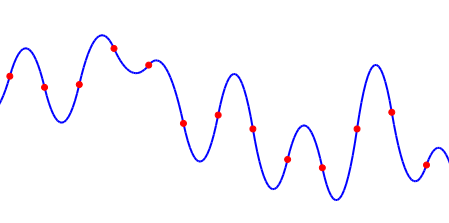
\includegraphics[width=0.8\textwidth]{img/rozkmit.png}\label{img:rozkmit}
	\caption{Nežádoucí rozkmit kvadratického spline}
\end{figure}

\section{Akima spline}

Akima spline je speciální formou kubického spline. Stejně jako kvadratický spline tvoří i Akima spline spojitě diferencovatelnou křivku, což opět zaručuje zachování derivací zleva a zprava v každém bodě.

Obecnou kubickou funkci lze zapsat rovnicí

\begin{equation}\label{eq:cubic}
f(y)=ax^3+bx^2+cx+d,
\end{equation}

pro Akima spline byla však tato definice upravena jako

\begin{equation}
f(y)=a(x-x_i)^3+b(x-x_i)^2+c(x-x_i)+d
\end{equation}

a to čistě jen proto, aby se zvýšila odolnost proti chybám vzniklým reprezentací čísel s plovoucí desetinnou čárkou. Ve vzorci totiž $x_i$ patří referenčnímu uzlu nalevo, takže dochází k redukci hodnot. S tím musí ovšem počítat i výpočet parametrů, jelikož křivka musí být posunuta tak, aby žádané hodnoty byly v intervalu $\langle0 ; x_{i+1} - x_i \rangle$

Celá metoda zakládá na odhadu sklonu křivek v závislosti na vstupních datech. Tyto elementární odhady jsou stanoveny pomocí sklonů přímek které prochází po sobě jdoucími body:

\begin{equation}
m_{i} = f'(x_{i})=\frac{y_{i+1} - y_i}{x_{i+1} - x_i}
\end{equation}

Odhady sklonů jsou posunuty o 2 hodnoty doleva, aby bylo možné symetricky interpolovat křivkami v každém bodě. Mimo to jsou první dvě váhy s indexy $-1$ a $-2$ a poslední dvě váhy za rozsahem hodnot $n$ a $n+1$ odhadnuty:

\begin{equation}
\begin{array}{rcl}
    m_{-1} & = & 2 m_0 - m_1 \\
    m_{-2} & = & 2 m_{-1} - m_0 \\
    m_{n}  & = & 2 m_{n-1} - m_{n-2} \\
    m_{n+1} & = & 2 m_{n} - m_{n-1} \\
\end{array}
\end{equation}

Dále jsou stanoveny vážicí koeficienty pro každý úsek jako:

\begin{equation}
\begin{array}{rcl}
 w_{i+1} & = & |m_{i+2} - m_{i+1}| \\
 w_{i-1} & = & |m_{i} - m_{i-1}| \\
\end{array}
\end{equation}

Finální rovnice pro koeficienty Akima spline křivky:

\begin{equation}
\begin{array}{rcl}
 d_i & = & y_i \\
 c_i & = & \frac{(w_{i+1} * m_i + w_{i-1} * m_{i+1})}{w_{i+1} + w_{i-1}} \\
 b_i & = & \frac{3 m_i - 2 a_i - c_{i+1}}{x_{i+1} - x_i} \\
 a_i & = & \frac{c_i + c_{i+1} - 2 * m_i}{(x_{i+1} - x_i)^2}\\
\end{array}
\end{equation}

\subsection*{Výhody a nevýhody}

Hlavní výhodou metody Akima spline je mimo to, že přejímá výhody interpolace a spline křivek obecně hlavně to, že odstraňuje nedostatek který vykazuje kvadratický spline v podobě nepřirozeného rozkmitu. Akima spline je také konstruován tak, aby co nejvěrněji napodoboval manuálně interpolovanou křivku lidmi.

Nevýhodou je mírně větší složitost výpočtu parametrů, tedy i mírně větší výpočetní náročnost. Stále ale jde o poměrně jednoduchou metodu s velmi příznivými výsledky.

\section{Hermite spline}

Jedná se o další variantu kubického spline, obecný předpis je proto stejný jako v rovnici \ref{eq:cubic}. Stejně jako u ostatních polynomiálních spline jde o spojitě diferencovatelnou křivku.

Metoda je postavená na lineární kombinaci bázových funkcí, kterými jsou:

\begin{equation}
\begin{array}{rcl}
 h_{00} & = & 2t^3 - 3t^2 + 1 \\
 h_{01} & = & -2t^3 + 3t^2 \\
 h_{10} & = & t^3 - 2t^2 + t \\
 h_{11} & = & t^3 - t^2 \\
\end{array}
\end{equation}

na intervalu $\langle0;1\rangle$.

Funkce $h_{00}$ má v čase $t = 0$ hodnotu 1, funkce $h_{01}$ hodnotu 0, v čase $t = 1$ je tomu přesně naopak. Tato vlastnost se dá využít pro aplikování principů interpolace, a sice že křivka prochází krajními body. Funkce $h_{00}$ tedy bude násobit souřadnice levého bodu, funkce $h_{01}$ pravého. Zbývající funkce mají v hraničních bodech intervalu hodnotu 0, proto nemohou ovlivnit hodnotu výsledné lineární kombinace. Používají se pro násobení odhadovaných derivací v krajních bodech.

Pro zjednodušení výpočtu a možnosti převést tento výpočet do programového kódu je vhodné provést formální zápis pomocí matic a vektorů. Bázová matice $B$ složená z bázových funkcí vypadá takto:

\begin{center}
\begin{math}
B = 
 \begin{pmatrix}
  2 & -2 & 1 & 1 \\
  -3 & 3 & -2 & -1 \\
  0 & 0 & 1 & 0 \\
  1 & 0 & 0 & 0
 \end{pmatrix}
\end{math}
\end{center}

Pro násobení funkcí krajními body a derivacemi lze stanovit vektor těchto hodnot:

\begin{center}
\begin{math}
S = 
 \begin{pmatrix}
  P_i \\
  P_{i+1} \\
  T_i \\
  T_{i+1}
 \end{pmatrix},
\end{math}
\end{center}

kde $P_i$ je hodnota jedné ze souřadnic bodu levého, $P_{i+1}$ stejné ze souřadnic bodu pravého, $T_i$ je odhad derivace v levém bodě a $T_{i+1}$ v pravém.

Vektor výsledných parametrů pak lze zapsat jako produkt násobení vektoru:

\begin{equation}
Q = B \cdot S
\end{equation}

Hodnotu funkce v daném čase $t$ pak lze vyjádřit jako

\begin{equation}
Q = \begin{bmatrix}
  t^3 & t^2 & t & 1
 \end{bmatrix} \cdot B \cdot S
\end{equation}

Metod odhadu derivací v bodě existuje několik, ze standardně používaných lze uvést hlavně kardinální spline variantu, kde hodnota derivace v každém bodě je vyjádřena rovnicí

\begin{equation}
T_k = (1 - c)\frac{P_{k+1} - P_{k-1}}{t_{k+1} - t_{k-1}},
\end{equation}

kde parametr $c$ vyjadřuje pnutí v každém z krajních bodů intervalu. Tento parametr by měl nabývat hodnot z intervalu $\langle0 ; 1 \rangle$, není to však podmínkou.

Pro $c = 0.5$ jde o základní Catmull-Rom spline.

\subsection*{Výhody a nevýhody}

Hermite spline spočívají zejména v interpolaci ve více rozměrech, což není v našem případě příliš využito. Dále neobsahuje zákmity jako spline kvadratický a je možné volně parametrizovat pnutí v každém bodě.

Výpočet je ale mírně složitější zejména proto, že je potřeba provádět výpočet ve dvou rozměrech odděleně, a to jak při stanovení koeficientů, tak posléze při získání hodnoty v konkrétním bodě. Další nevýhodou je absence úseku prvního a posledního úseku křivky, což je dáno charakterem interpolační metody, kdy pro výpočet parametrů křivky v jednom úseku jsou třeba vlastnosti úseku předchozího a následujícího.

\section{Centripetal Catmull-Rom spline}

Catmull-Rom spline interpolační metody jsou podmnožinou Hermite spline metod. Použití metody Catmull-Rom je často v rovinných nebo prostorových interpolacích, například pro věrné napodobení cest mezi body při generování cesty, typicky v počítačových hrách. Pro obyčejnou funkční aproximaci ji použít však lze.

Catmull-Rom spline vyžaduje pro interpolaci jednoho segmentu 4 body, které jsou použity pro výpočet parametrů funkcí pro generování křivky mezi body prostředními. Do interpolačního procesu lze zanést parametrizaci v podobě stanovení parametru zvaného \uv{uzlový parametr} značeným $\alpha$ (často převáděný na parametr pnutí $\tau$), kterým lze snadno manipulovat s vlastnostmi křivky. Základní je parametrizace uniformní ($\alpha = 0, \tau = 0.5$), dále je pak často využívaná chordálová ($\alpha = 1, \tau = 0$), ovšem pro potřeby této práce je nejzajímavější parametrizace \emph{centripetal} ($\alpha = 0.5, \tau = 0.25$).

Centripetal parametrizace odstraňuje z uniformní křivky protínání sebe sama a narozdíl od chordálové se těsněji přibližuje vstupním datům a tak vytváří křivku, která je věrnější. Také lze chordálovou a centripetal Catmull-Rom v případě interpolace funkce hodnoty závislé na čase převést na funkci. Uniformní parametrizace by mohla porušit vlastnosti funkcí i v případě bodů které v seřazené posloupnosti mají pouze rostoucí hodnotu $x$. Centripetal parametrizace je pak první, která vlastnosti funkce neporušuje. Chordálová pak tvoří výrazné oblouky kolem interpolovaných bodů, které mohou v případě funkční interpolace být nežádoucí.

Nejdříve je třeba vypočíst vážené vzdálenosti bodů pomocí parametru $\tau$:

\begin{equation}
\begin{array}{rcl}
 dt_{i} & = & ((x_{i+1} - x_i)^2 + (y_{i+1} - y_i)^2)^\tau \\
\end{array}
\end{equation}

a následně vypočítat časovou parametrizaci pro finální stanovení koeficientů pro křivku v daném segmentu:

\begin{equation}
\begin{array}{rcl}
 T_i & = & dt_{i} ( \frac{P_{i+1} - P_i}{dt_{i}} - \frac{P_{i+2} - P_i}{dt_{i} + dt_{i+1}} + \frac{P_{i+2} - P_{i+1}}{dt_{i+1}} ), \\
\end{array}
\end{equation}

kde $P$ je jedna ze souřadnic $x$ nebo $y$. Výsledné hodnoty $T_i$ a $T_{i+1}$ společně se vstupními body $P_i$ a $P_{i+1}$ lze následně dosadit do vztahů Hermite spline.

\subsection*{Výhody a nevýhody}

Catmull-Rom spline v parametrizaci centripetal v podstatě sdílí výhody a nevýhody s Hermite spline.

Jediným větším rozdílem oproti základnímu Hermite spline je složitější výpočet odhadu derivace ve vstupních bodech, který vede ve větší \uv{volnost} v každém z nich. To opět může být pro některé aplikace žádoucí.



\chapter{Implementace}

V této části bude popsána kostra zpracování aplikace a budou rozebrány významné problémy, které byly při implementaci řešeny.

\section{Načítání dat}

Načítací vrstva byla vytvořena tak, aby odpovídala zbytku aplikace, který z velké části sestává z předpřipravené kostry poskytnuté přednášejícím. Jelikož je využíván princip rozhraní, respektive abstraktních tříd s čistě virtuálními metodami, byl tento přístup dodržen i zde.

Základním rozhraním pro práci s úložištěm je rozhraní \texttt{ILoader}, které obsahuje metody \texttt{InitLoader}, \texttt{LoadGlucoseLevels} a \texttt{Finalize}. Metoda \texttt{InitLoader} provede načtení zdroje se zadanými parametry, ověří správnost zdroje a jeho formátu. Metoda \texttt{LoadGlucoseLevels} slouží k načtení dat ze zdroje do cílového vektoru po segmentech, aby bylo možné rovnou provádět požadované operace. Metoda \texttt{Finalize} pak zdroj korektně uzavírá a uvolňuje alokovanou paměť.

V konkrétním případě byla implementována třída \texttt{SQLiteLoader}, která tyto metody implementuje ve variantě pro SQLite3 souborovou databázi.

\section{Výpočet parametrů}

Výpočet parametrů je mnohem specifičtější a komplikovanější část programu. Vzhledem ke snaze mít program optimální bylo zavedeno několik opatření, která redukují počet operací, které je nutné provést v průběhu výpočtu.

\subsection{Rozhraní}

Jak bylo vyžadováno ve vzoru, všechny interpolační metody jsou implementovány v samostatných třídách, které dědí od společného předka\\ \texttt{CCommonApprox}. Implementují proto metody \texttt{Approximate}, \texttt{GetLevels} a nově po individuální domluvě i metodu \texttt{GetBounds}. Konstruktor každé třídy přejímá vstupní data, tedy naměřené hodnoty načtené do připravených přepravek odděděných od abstraktní \texttt{IGlucoseLevels}. Metoda \texttt{Approximate} přejímá vstupní parametry pro metodu a stará se o samotný výpočet parametrů interpolující křivky. Jedná se tedy o metodu, kde je nutné běh algoritmu paralelizovat dle zadaných kritérií. Metoda \texttt{GetLevels} pak pro zadaný rozsah provede vyhodnocení předvypočtených křivek a vrací hodnotu v požadovaných bodech. Metoda \texttt{GetBounds} slouží pro výpočet výsledného rozsahu vstupních dat, který byl k interpolaci použit. To je vhodné pro interpolační metody, které potřebují k aproximaci jednoho úseku více, než dva hraniční body, a tedy nemohou interpolovat například první a poslední úsek křivky (tedy oblast mezi nultým a prvním bodem, případně předposledním a posledním).

Všechny tyto metody mají návratový typ \texttt{HRESULT}, který dovoluje ohlásit chybový stav v případě, že byly použity neplatné parametry. Pokud nedošlo k chybě, metody vrací \texttt{S\_OK}. Pokud však k chybě došlo, je vrácena hodnota \texttt{S\_FALSE}. Typicky takový stav nastane, když je do interpolační metody předán neplatný parametr na vstupu, nebo pokud požadujeme hodnotu interpolační křivky v bodě, ve kterém kvůli vstupním datům hodnota neexistuje.

\subsection{Algoritmus}\label{algo:impl}

Hovoříme-li o paralelizaci na úrovni masek, samotný algoritmus je rámcově jiný pro sériový a pro paralelní výpočet. U sekvenčního výpočtu se totiž můžeme spolehnout, že bude výpočet parametrů prováděn na po sobě jdoucích bodech, tedy je možné použít menší režii kolem rozhodování, odkud data brát, případně kam je uložit. Paralelní algoritmus však dostane přidělenou práci dynamicky z nějakého obecného poolu, tedy nemusí jít o po sobě jdoucí body, resp. bloky bodů.

\subsubsection*{Předvypočítané hodnoty}

Sériový algoritmus tedy může využívat předvypočtenou sadu offsetů, ve které bude se bude pouze posouvat pomocí jedné inkrementující proměnné. Například mějme masku $154_{(10)}$, tedy $10011010_{(2)}$. Pro takovou masku víme, že se bude tento vzor opakovat v rámci oktetu po sobě jdoucích hodnot v segmentu. Z tohoto vzoru je zřejmé, že se budou opakovat offsety $0$, $3$, $4$, $6$, jen se bude jednou za $N$ hodnot posouvat báze, kde $N$ je váha masky (počet jednotek v binárním oktetu, zde $4$). Vykonstruované pole tedy má základní tvar \texttt{[0,3,4,6]}, který ovšem není finální. Tento tvar by dostačoval v případě, že bychom potřebovali přistupovat k právě jednomu prvku za celou dobu výpočtu, a nepotřebovali bychom žádný kontext. To ale v žádném případě interpolačních metod neplatí, a proto je nutné pole rozšířit. Kvadratický spline vyžaduje alespoň jeden prvek následující, Akima spline vyžaduje jeden následující, ale k předvýpočtu derivací je zapotřebí dvou dalších, Catmull-Rom a Hermite spline však vyžadují největší kontext, a sice jednoho bodu vlevo a dvou vpravo od současného. Tento kontext lze převést i na libovolnou variaci vzniklou posuvem, a proto budeme potřebovat kromě jednoho prvku vždy 3 následující. V každém bodě základní sady (zde 4 hodnoty) bude třeba uchovávat tedy alespoň o 3 pozice více. Ty vzniknou cyklickým opakováním masky tak, že vezmeme první 3 prvky pole a zvětšíme je o velikost oktetu, tedy $8$. Výsledkem je tedy pole \texttt{[0,3,4,6,8,11,12]}. Musíme ale počítat s různými vahami masek, proto všechna takto předvypočtená pole budou muset mít předem stanovenou pevnou délku danou největší vahou, tedy vahou $8$. Pole musíme proto rozšířit na $8 + 3$ prvků, tedy $11$. Předvypočtené hodnoty všech těchto polí lze nalézt v souboru \texttt{precalculated.h} pod názvem \texttt{mask\_shift\_base}, což je pole o $256$ prvcích, kde se pro každou masku nachází právě jedno předvypočtené pole posuvů.

Pro účely paralelních algoritmů je využito pole obdobné s názvem\\ \texttt{mask\_index\_transform}, které však obsahuje pouze $8$ prvků vzhledem k tomu, že lze každý prvek spočítat se stejnou složitostí včetně stejného charakteru operací. Pole je menší, což zvyšuje pravděpodobnost setrvání větší části v nižších úrovních cache CPU, což může přinést jisté urychlení vzhledem k tomu, že je využito více výpočetních jader, kde každé má svou hierarchii cache.

Kromě těchto polí je dále předvypočteno pole \texttt{mask\_weights}, které obsahuje předvypočtené váhy masek. Ty jsou vždy konstantní a není třeba je přepočítávat při každém běhu programu nebo algoritmu znovu.

\subsubsection*{Ukládání vypočtených parametrů}

Vypočtené parametry jsou ukládány do kondenzovaného pole, kde každému úseku křivky náleží právě jeden index. Zároveň se lze spolehnout, že po sobě jdoucí úseky mají po sobě jdoucí indexy v kondenzovaném poli.

Zde ale vyvstává problém, jak efektivně dojít ke kondenzaci pole za běhu. Jednotlivým workerům je přidělován jako kus práce index do kondenzovaného pole. Každý worker si proto musí vypočítat index použitých hodnot v poli se všemi hodnotami, a to podle rovnice \ref{eq:kondenzace}.

\begin{equation}\label{eq:kondenzace}
i = 8 \cdot\left\lfloor\frac{i_{k}}{w_{mask}}\right\rfloor + tr_{mask}[i_{k} \bmod w_{mask}],
\end{equation}
kde $i_{k}$ je index v kondenzovaném poli, $w_{mask}$ váha masky a $tr_{mask}$ je odpovídající index v poli \texttt{mask\_index\_transform}.

První člen v rovnici vypočte bázový index, který lze odvodit poměrově. Je-li váha masky $4$, znamená to, že každý oktet je zredukován na čtyři prvky. Lze tedy říct, že každým $8$ prvkům v nekondenzovaném poli náleží $4$ v poli kondenzovaném.

Druhý člen poté provádí transformaci offsetu, který zakládá na předvypočtených hodnotách v poli \texttt{mask\_index\_transform}.

\section{Implementace interpolačních metod}

Všechny algoritmy pro výpočet vybraných interpolačních křivek zakládají na metodách uvedených v předchozí podkapitole. Ty ale řeší problém přístupu k paměti a efektivitu režie kolem výpočtu, ne ale výpočet samotný.

Výpočet je vždy specifický pro každou interpolační metodu a má oddělenou implementaci. Stejně tak má v rámci metody oddělenou implementaci každý způsob parametrizace.

V metodě \texttt{Approximate} rozhraní \texttt{IApproximatedGlucoseLevels} implementované v rámci každé interpolační metody se nachází větvení, které rozhodne na základě vybraného způsobu paralelizace, kterou metodu zavolá. V případě sériového výpočtu je volána pouze ve smyčce metoda \texttt{\justify CalculateParametersForMask(uint8\_t mask)}, pro použití vláken \texttt{\justify CalculateParameters\_threads()}, pro Intel TBB \texttt{\justify CalculateParameters\_TBB()} a pro OpenCL \texttt{\justify CalculateParameters\_OpenCL()}.

Konkrétní podobu těchto funkcí zde nemá smysl uvádět, jelikož jsou v podstatě přepisem matematických rovnic odvozených v kapitole \ref{mat:main}, pouze s dodatkem v podobě paralelizace.

Metoda kvadratického spline paralelizuje vždy na úrovni segmentů (každý worker jednu masku). Ostatní metody to v rámci paralelizace pomocí Intel TBB dělají také, ale pouze do určité hranice počtu bodů, jelikož do této hranice by režie přidělování práce napříč maskami způsobila spíše snížení efektivity. Zbytek výpočtů je prováděn na úrovni masek, tedy každý worker počítá parametry pro právě jeden úsek křivky v jedné masce v jeden čas.

\section{Výpočet hodnoty v bodě}

K výpočtu hodnot v bodě, a to jak po jednom, tak hromadně, slouží metoda \texttt{\justify GetLevels} rozhraní \texttt{\justify IApproximatedGlucoseLevels}.

Pro výpočet hodnoty v bodě je třeba jednak vybrat správný úsek křivky v závislosti na vstupních datech a aktuální masce, a jednak dopočíst správný index referenčního uzlu, který většina metod vyžaduje. K tomu má každá třída představující interpolační metodu implementovanou metodu \texttt{\justify GetIndexFor}, která v případě, že požadovaná hodnota je v intervalu interpolovaných křivek naplní potřebné indexy z pole hodnot a vrátí \texttt{S\_OK}. V případě že ne, vrací \texttt{S\_FALSE}.

Index ve vstupních datech je následně převeden pomocí předvypočteného pole \texttt{\justify mask\_index\_transform\_inverse} na index správného úseku křivky.

Následně je cyklicky za použití masky a soustavného posouvání indexu pomocí pole \texttt{\justify mask\_shift\_base} naplněno pole interpolovaných hodnot, a to pomocí předvypočtených parametrů křivek a obecných předpisů funkcí pro každou metodu, kam je dosazena aktuální hodnota nezávislé proměnné.

Nezávislou proměnnou je v případě kvadratického a Akima spline samotné $x$, jakožto i vstupní parametr metody \texttt{\justify GetLevels}, do Hermite a centripetal Catmull-Rom spline však vstupuje parametr času. Ten je třeba zpětným řešením rovnic vyjádřit. Jelikož si u obou těchto metod můžeme být jisti, že parametr času $t$ lze vypočíst z kubické rovnice pro souřadnici $x$, stejně jako že pro každou hodnotu $x$ z intervalu $\langle 0 ; 1 \rangle$ existuje právě jedna hodnota $t$ z téhož intervalu, lze rovnici řešit klasickou metodou pro řešení kubických rovnic, ale použít pouze první reálný výsledek (bez imaginární části), který spadá do tohoto intervalu. Ten bude vždy právě jeden.

\section{Výpočet statistik}

Výpočet statistik je zcela odděleným procesem z pohledu aplikace. Pro každý bod vstupních dat je volána metoda \texttt{\justify GetLevels}, a to pro naplnění jedné konkrétní hodnoty, pomocí které je spočtena absolutní a relativní chyba, a následně dalším voláním i hodnota derivace, kde je zkoumána chyba absolutní. Postupně jsou takto naplněna tři dvourozměrná pole hodnot, představující absolutní a relativní chyby interpolovaných hodnot každého bodu v každé masce a absolutní chyby derivace v každé masce.

Z těchto hodnot jsou poté vypočteny požadované statistické ukazatele - minimální, maximální, průměrná chyba, medián, 1. a 3. kvartil a standardní odchylka chyby. Tyto ukazatele jsou naformátovány do klasického CSV formátu a vypsány na standardní výstup. Na závěr je vypsána informace o tom, zdali je metoda interpolace spojitě diferencovatelná, což zahrnuje i informaci o tom, zda má spojitou derivaci. V případě všech implementovaných metod je tato vlastnost splněna.

\chapter{Uživatelská dokumentace}

\section{Sestavení programu}

\section{Ovládání programu, parametry}




\chapter{Výsledky}

\section{Zhodnocení interpolačních metod}

\section{Porovnání algoritmů}

\section{Metriky}

\subsection{Amdahlův zákon}

\subsection{Gustavsonův zákon}

\subsection{Karp-Flattova metrika}




\chapter{Závěr}




\end{document}
